\documentclass[11pt,a4paper]{article}
\input{article-recherche}
% Macros locales pour le Scénario 2
\newcommand{\stab}{\mathrm{stab}}
\newcommand{\rang}{\mathrm{rk}}


\title{Note de travail : Stabilité d'un opérateur discret}
\author{Chercheur (Exemple d'entraînement)}
\date{\today}

\begin{document}
\maketitle

\section{Contexte}
Les méthodes récentes d'assistance formelle en Lean 4 permettent de vérifier des preuves longues [À CITER : article récent sur l'autoformalisation en Lean 4].

\section{Résultat principal}
\begin{definition}[Domaine admissible]
On se place pour tout entier naturel $n \ge 1$.
\end{definition}

\begin{lemma}[Majoration de stabilité]
Pour tout entier $n \ge 1$, l'indice de stabilité $\stab(n)$ vérifie $\stab(n) \ge 1$.
\end{lemma}

\begin{proof}
Pour $n \ge 2$, la propriété découle d'un calcul direct.
\unproven{Vérifier séparément le cas limite $n = 1$.}
\end{proof}

\section{Diagramme illustratif (avec chevauchement volontaire)}
\begin{center}
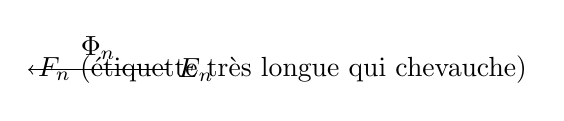
\begin{tikzpicture}
  \node (A) at (0,0) {$E_n$};
  \node (B) at (1.1,0) {$F_n$ (étiquette très longue qui chevauche)};
  \draw[->] (A) -- node[above] {$\Phi_n$} (B);
\end{tikzpicture}
\end{center}

\bibliographystyle{plain}
\bibliography{references}
\end{document}
